\chapter{关键操作(方法)函数的实现} 
% \pagenumbering{arabic} % 阿拉伯数字页码
% 与第五部分有所对应,用带注释伪码论述
% 一些例子,可以模仿。

\section{GDT与IDT表项的设置}
GDT和IDT的设置还是相对还是比较复杂的,因为这很大程度上是由x86硬件决定的,
个人不能自由发挥,需要查阅相关手册,了解硬件设计的结构,依此来编写代码.
更麻烦的是,由于x86要考虑兼容性,一些本来简单的几个数据项能要拆成几段,"身首异处",
这就需要我们在设置的时候大量采用位操作,把数据项该拆的拆,该还原的还原,放到他们应放的地方去.
这部分建议阅读赵炯《Linux内核完全剖析》以及osdev网站上有关x86硬件的介绍,维基百科上亦有相关资料
(https://en.wikipedia.org/wiki/Global\_Descriptor\_Table).
\subsection{GDT}
GDT表项高32位如下,granularity粒度位G这里设为1,AVL为系统可用位.

\begin{tabular}{|c|c|c|c|c|}% 通过添加 | 来表示是否需要绘制竖线
    % \toprule
    % Exception \# & Description & Error Code?\tabularnewline
    \midrule
    23 & 22 & 21 & 20 & 19 - 16\tabularnewline
    G  &D/B & L  &AVL & 段界限 \tabularnewline
    1  &1   & 0  &   &        \tabularnewline
    \bottomrule
\end{tabular}

赵炯《Linux内核完全剖析》P91 数据段和代码段在TYPE段的不同编码:


\begin{tabular}{|c|c|c|c|c|}% 通过添加 | 来表示是否需要绘制竖线
    % \toprule
    % Exception \# & Description & Error Code?\tabularnewline
    \midrule
         &        &    &<-  TYPE ->& \tabularnewline 		
     15 & 14-13  & 12 &   11 - 8   & 7 - 0\tabularnewline     
    \bottomrule
\end{tabular}


\begin{tabular}{|c|c|c|c|c|}% 通过添加 | 来表示是否需要绘制竖线
    % \toprule
    % Exception \# & Description & Error Code?\tabularnewline
    \midrule
    data segment:& p &  DPL  & 1 & 0 E W A   \tabularnewline 
    code segment:& p &  DPL  & 1 & 1 C R A   \tabularnewline    
    \bottomrule
\end{tabular}


其中一些字母的含义为: 

E:扩展方向,W:可写,A:已访问,C:一致代码段,R:可读

这部分原理理解起来不是很困难,然而要保证一个位都不能错,否则系统还是不会正常工作,
在位操作的过程中我们可能弄晕了,忘了它本来面目是什么,网站https://wiki.osdev.org/GDT\_Tutorial
提供了一个简单的小程序,我们通过它可以事先算出GDT设置好后是什么样,可以和我们自己用位操作搞出来的GDT
表项的值相互验证,例如运行在ring0和ring3的代码段和数据段应该怎样设置:

\begin{tabular}{|c|c|}% 通过添加 | 来表示是否需要绘制竖线
    \toprule
    值 & 含义\tabularnewline
    \midrule
    0x0000000000000000 & NULL \tabularnewline 
    0x00CF9A000000FFFF & GDT CODE PL0 \tabularnewline 
    0x00CF92000000FFFF & GDT DATA PL0 \tabularnewline 
    0x00CFFA000000FFFF & GDT CODE PL3 \tabularnewline 
    0x00CFF2000000FFFF & GDT CODE PL3 \tabularnewline  
    \bottomrule
\end{tabular}

\subsection{IDT}
IDT表项的设置也应该依据IDT结构图来进行相关位操作,下面是如何把对应的值设置到中断门描述符的操作过程,
陷阱门描述符的设置也与之类似.
\begin{minted}{c}
void set_interrupt_gate(struct GATE_DESCRPTOR *descr, u16 index ,u32 offset, u8 dpl)
{
descr->offset_lowerbits = offset & 0xffff;
descr->selector = index << 3;/*the lower 3 bits is TI(2) and RPI(0,1)*/
descr->zero = 0x00;
descr->seg_type = Gate_INTERRUPT_TYPE;/*0x0E*/
descr->storage = 0b0;
descr->descr_privilege_level = dpl;
descr->present =0b1;
descr->offset_higherbits = (offset & 0xffff0000) >> 16;
}
\end{minted}


\section{成组链接}

\begin{figure}[!htbp]
		\centering	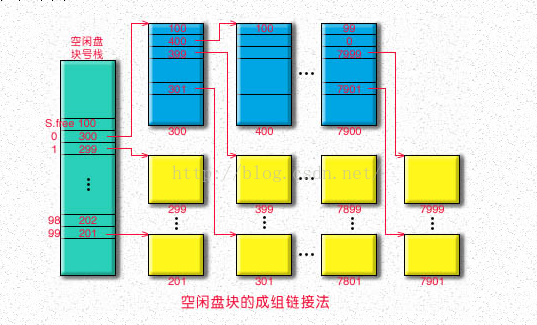
\includegraphics[width=14cm]{pic/assets/grouping}
		\caption{成组链接原理}	\label{grouping}	\end{figure}
		
初始化时,若之前未初始化,先指定第一组的第一块为专用块,把此块复制到内存专用块中;
如果已经初始化,从磁盘加载超级块到内存,得到专用块的块号.

所有组的第一块相互链接,类似一个顺序表,这些组的第一块第一项存空闲块计数,第二项存下一块的块号,
当专用块用完时,它就指定它的下一块是专用块,并在超级块中更改专用块的块号.成组链接原理图来自CSDN.

关于组号,写代码时从0开始编号,0到127,开始的几组如图~\ref{grouping_1}~所示.	

\begin{figure}[!htbp]
		\centering	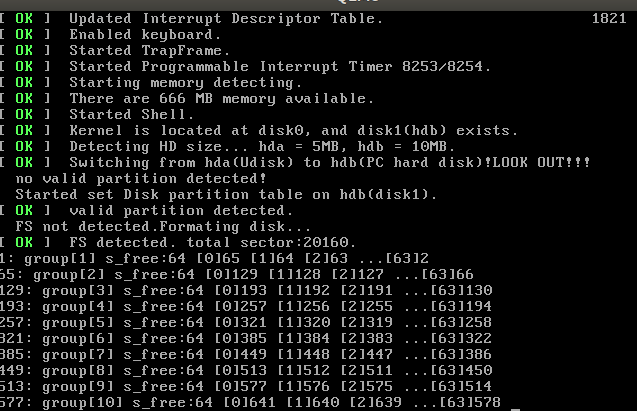
\includegraphics[width=14cm]{pic/assets/grouping_1}
        \caption{grouping(1)}	\label{grouping_1}	\end{figure}
        
末尾的几组如图~\ref{grouping_2}~所示.	

\begin{figure}[!htbp]
		\centering	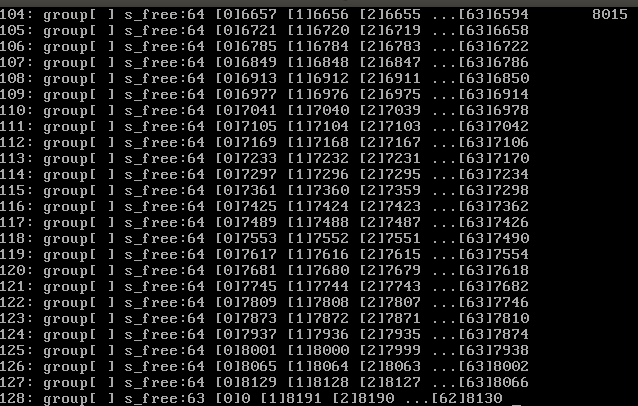
\includegraphics[width=14cm]{pic/assets/grouping_2}
		\caption{grouping(2)}	\label{grouping_2}	\end{figure}

注意,最后一组空闲块要少一个,而且最后一组没有下一组,s\_free\_blk\_nr[0] = 0;即下一组不存在.

第一次进入rios系统时,系统探测到磁盘上超级块的固定区域没有magic number判断出rifs尚未被建立,
故格式化硬盘,建立硬盘分区表,建立根目录.调用read和write将文件内容写入txt文件并读出到屏幕上显示.

第一次如图~\ref{first_rios}~所示.	

\begin{figure}[!htbp]
		\centering	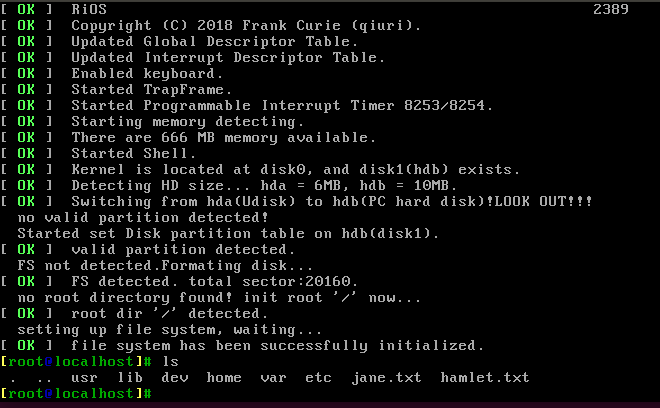
\includegraphics[width=14cm]{pic/assets/first_rios}
		\caption{第一次进系统}	\label{first_rios}	\end{figure}

下次进系统如图~\ref{next_rios}~所示.第二次(或以后)进入系统时,已经检测到magic number的存在,
故不再格式化磁盘,调用ls命令可见当前根目录下系统已经在上一次建立好了一些默认的文件夹,
而且并不会随着关机再开机而丢失,系统中我已经编写了键盘驱动和屏幕字符显示驱动,随着键盘敲击,
命令送入缓冲区,敲击回车时,命令送入命令解释程序即shell中解释运行,系统中先后调用
ls,cd qiuri,cd ..,pwd,mkdir dir1/dir2/dir3,cd dir1/dir2/dir3等,
可以看到测试效果良好,没有问题.	

\begin{figure}[!htbp]
		\centering	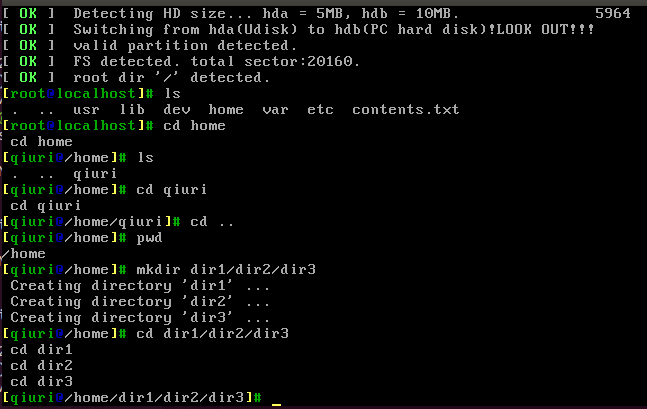
\includegraphics[width=14cm]{pic/assets/next_rios}
		\caption{下次进系统}	\label{next_rios}	\end{figure}


\subsection{空闲磁盘块的成组链接分配与回收方法}

成组链接方法是应该能够将之前的专用块(若闲置)给分配出去的,
上图是我不断申请新块,并将块号打印出来的情况,
可见我在分配了64号即第一组除了下一组之外的最后一个空闲块之后,开始转入第二组,
并从第二组中分配空闲块,然后下一次分配就能把之前的专用块(现已闲置)给分配出去,
即把1号分配出去了.如此下去,将如抽丝一般把整个磁盘上的磁盘块(包括不用的前专用块)给分配出去,

因为在做文件系统之前,我已经实现了设备管理,编写了IDE硬盘的驱动,
因而可以读写任意扇区,这里封装了hexdump 命令,可以把磁盘上任意一个扇区内容以十六进制打印出来,
从info disk命令中我们知道数据区从第521扇区开始,因为我们采取成组链接,
也按一定规律初始化了,故数据区第一个扇区的是存成组链接信息的.
在RiOS中数据区一个块两个扇区,故第一个有效的空闲区是第523扇区.该扇区用作某目录的数据区,图可见之前的.


\subsection{初始化}

为了基于空闲磁盘空间的成组链接方式的初始化,系统中有一个自定义的磁盘块联合体free\_space\_grouping\_head:

\begin{minted}{c}
union free_space_grouping_head {/*成组链接法,各组空闲块的头*/
	u16 bytes[512] = {0};/*占坑位 2 sectors*/
	struct {
		u16 s_free;
		u16 s_free_blk_nr[BLKS_PER_GROUP];/*[64]*/
	};
/*s_free_blk_nr[0] is next free group's nr*/
};	
\end{minted}

在rifs中,对于数据区,空闲磁盘空间管理采用成组链接方式,一个磁盘数据块有两个扇区,
这里采用了联合体而不是结构体,意义主要在于占位,使得一个这样的联合体恰好1024B即
两个扇区即一个数据块的大小,若此磁盘块为组里第一块,则它要记录整个组空闲块的信息,
第一项s\_free记录本组共有几个空闲块,其后的表项记录本组所有空闲块的块号,
其中s\_free\_blk\_nr[0]记录下一组的组号,若已经是最后一组,则s\_free\_blk\_nr[0]=0,
每次分配时s\_free-=1,然后以s\_free为数组下标,找到s\_free\_blk\_nr[]相应的空闲块号,
即为要分配的块号.若s\_free-=1后为0时,找下一组调入专用块,到下一组去找空闲块.


\section{目录项的确定}
如何得知一个目录文件里有多少个目录项?目录文件的inode中记录有大小i\_size,
由目录文件的inode中的i\_size得到目录文件大小.而struct dir\_entry目录项的大小是固定的,
由i\_size除以 sizeof(dir\_entry)可知有几个目录项目.

\section{多级索引}

教科书上Linux ext2多级索引原理示意图如图~\ref{Linux ext2 fs}~
\begin{figure}[!htbp]
	\centering	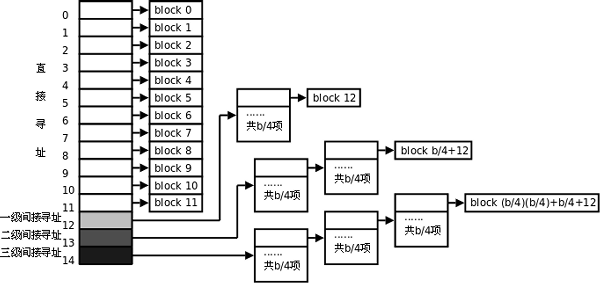
\includegraphics[width=14cm]{pic/assets/Linux_ext2_fs}
	\caption{Linux ext2}	\label{Linux ext2 fs}	\end{figure}

RiOS中的设定:

\begin{enumerate}
\item  zone[0~6]:	direct block 
\item  zone[7]:	    single indirect block
\item  zone[8]:	    double indirect block 
\item  zone[9]:	    trible indirect block
\end{enumerate}

大致估计一下容量.

\paragraph{直接寻址} zone[0~6]直接寻址: 

    每个块2扇区,7*(2*512)=7168B = 7kB

 length: 0~7(2512)B              [0,7168] B

 sector:length/512 	[1,7*2]

\paragraph{一次寻址} zone[7] 一次间址: 

    u16 zone[] u16 => 2B , 一个区可以存(2*512)/2=512 个扇区号,
    512 * (512*2) = 512kB.

 length: 7(2512)+1 ~ 7(2512)+512(5122) 

        [7169,531456]  B

 sector:$\left\lceil{length/512}\right\rceil$   $\sim$   [72+1,72+512*2]

[15,1038]      

\paragraph{两次寻址} zone[8] 两次间址: 512 * 512 * (512 * 2)= 256 MB 

 length:  7(2*512)+512(512*2)+1 $\sim$ 7(2512)+512(5122)+512512(512*2)

 	[531457,268966912] B

 sector:$\left\lceil{length/512}\right\rceil$  $\sim$    [72+5122+1,?]	

 	[1039,525326]

\paragraph{三次寻址} zone[9] 三次间址: 512 * 512 * 512 * (512 * 2) = 128 GB 

 length: 7*(2*512)+512 * (512 * 2)+512 * 512 * (512*2)+1 $\sim$  7*(2*512)+512(512*2)+512*512(512*2)+512 * 512 * 512 * (512 * 2)

[268966913,137707920384] B

三次间址理论上支持很大容量,但实际上做实验用不到那么多.

\subsection{删除文件}

删除文件相对来说比较麻烦,但不是很困难,但要仔细.分几种情况讨论,从直接寻址到一次寻址,
再到两次寻址,犹如一个分段函数.

\begin{minted}{c}   
void rm(const char *name,u8 mode)
{
	int fd = open(name);if(fd==-1)return;
	int contents_len = current->filp[fd]->f_inode->i_size;
	if( current->filp[fd]->f_inode->i_size==0){
		kprintf("\n rm: '%s': not a valid file.",name);
		return;
	}
	if(current->filp[fd]->f_inode->i_nlinks!=0)
		kprintf("\n rm: nlinks:%d",current->filp[fd]->f_inode->i_nlinks);
	u16 ino = current->filp[fd]->f_inode->i_ino;
	int length = current->filp[fd]->f_inode->i_size;
	close(fd);
	if(ino==0) _panic(" FBI WARNING:rm:i_ino = 0 !!! ");/* will destroy root directory */
/* free blocks and then free inode,finally remove this record from the directory */	
	u8 sector[512]={0};int buffer_offset=0;
	int total_sectors = (length+511)/512;
	struct m_inode rm_inode;
	iget(&rm_inode,ino);

	memset(sector,0x00,sizeof(sector));
	if(total_sectors<=7*SECTOR_PER_BLOCK){
/* @#0.1 zone[0~6]: direct block 直接寻址,大概7kB*/
		for(int i=0; i<total_sectors; i++){
			int blk_i = get_zone_blks(i+1)-1;
			if(i%2==0){
				IDE_write_sector((void *)&sector, DATA_BLK_NR_TO_SECTOR_NR(rm_inode.i_zone[blk_i]));
			}else{
				IDE_write_sector((void *)&sector, DATA_BLK_NR_TO_SECTOR_NR(rm_inode.i_zone[blk_i])+1);
				if(rm_inode.i_zone[blk_i]!=0)free_block(rm_inode.i_zone[blk_i]);	
			}
		}
	}else if(total_sectors<=7*SECTOR_PER_BLOCK+512*SECTOR_PER_BLOCK){
/* @#1.1 zone[0~6]: direct block 直接寻址,大概7kB*/		
		for(int i=0; i<7*SECTOR_PER_BLOCK; i++){
			int blk_i = get_zone_blks(i+1)-1;
			if(i%2==0){
				IDE_write_sector((void *)&sector, DATA_BLK_NR_TO_SECTOR_NR(rm_inode.i_zone[blk_i]));
			}else{
				IDE_write_sector((void *)&sector, DATA_BLK_NR_TO_SECTOR_NR(rm_inode.i_zone[blk_i])+1);	
				if(rm_inode.i_zone[blk_i]!=0)free_block(rm_inode.i_zone[blk_i]);
			}
		}
/*  #1.2 zone[7]:   single indirect block 一次间址,大概五百kB*/
		u8 two_sectors[1024]={0};/*load indexs in zone[7] to memory 'two_sectors'*/
		IDE_read_sector((void *)two_sectors, DATA_BLK_NR_TO_SECTOR_NR(rm_inode.i_zone[7]));
		IDE_read_sector((void *)(two_sectors + 512), DATA_BLK_NR_TO_SECTOR_NR(rm_inode.i_zone[7])+1);
		u16 * pzone =(u16 *)&two_sectors;/* that's right */

		for(int i = 7*SECTOR_PER_BLOCK;i<total_sectors;i++){//[7*2+1,7*2+512*2]
			int blk_i = get_zone_blks(i+1)-1;
			u16 zone_index = pzone[blk_i-7];/*zone[0~6]*/
/* MAKE SURE that zone_index!=0. assert(zone_index!=0)*/			
			if(zone_index==0) {
				_panic("FBI WARNNING:rm:zone_index should not be zero!!!");/* will destory root directory!*/			
			}
			if(i%2==0){
					IDE_write_sector((void *)&sector, DATA_BLK_NR_TO_SECTOR_NR(zone_index));
			}else{
					IDE_write_sector((void *)&sector, DATA_BLK_NR_TO_SECTOR_NR(zone_index)+1);
					if(zone_index!=0)free_block(zone_index);
			}
		}

		if(rm_inode.i_zone[7]!=0)free_inode(rm_inode.i_zone[7]);
	}
	else if(total_sectors<=7*SECTOR_PER_BLOCK+512*SECTOR_PER_BLOCK+512*512*SECTOR_PER_BLOCK){
/* @#2.1 zone[0~6]:  direct block 直接寻址,大概7kB*/	
		kprintf("\n  rm: removing direct blocks of file '%s'.",name);
		for(int i=0; i<7*SECTOR_PER_BLOCK; i++){
				int blk_i = get_zone_blks(i+1)-1;
				if(i%2==0){
					IDE_write_sector((void *)&sector, DATA_BLK_NR_TO_SECTOR_NR(rm_inode.i_zone[blk_i]));
				}else{
					IDE_write_sector((void *)&sector, DATA_BLK_NR_TO_SECTOR_NR(rm_inode.i_zone[blk_i])+1);	
					if(rm_inode.i_zone[blk_i]!=0)free_block(rm_inode.i_zone[blk_i]);
				}
		}
/*  #2.2 zone[7]  :  single indirect block 一次间址,大概五百kB*/
		kprintf("\n  rm: removing single indirect blocks of file '%s'.",name);
		u8 two_sectors[1024]={0};/*load indexs in zone[7] to memory 'two_sectors'*/
		IDE_read_sector((void *)two_sectors, DATA_BLK_NR_TO_SECTOR_NR(rm_inode.i_zone[7]));
		IDE_read_sector((void *)(two_sectors + 512), DATA_BLK_NR_TO_SECTOR_NR(rm_inode.i_zone[7])+1);
		u16 * pzone =(u16 *)&two_sectors;/* that's right */

		for(int i = 7*SECTOR_PER_BLOCK;i<7*SECTOR_PER_BLOCK+512*SECTOR_PER_BLOCK;i++){//[7*2+1,7*2+512*2]
			int blk_i = get_zone_blks(i+1)-1;
			u16 zone_index = pzone[blk_i-7];/*zone[0~6]*/
/* MAKE SURE that zone_index!=0. assert(zone_index!=0)*/			
			if(zone_index==0) {
				_panic("FBI WARNING:read:zone_index should not be zero!!!");/* will destory root directory!*/			
			}
			if(i%2==0){
					IDE_write_sector((void *)&sector, DATA_BLK_NR_TO_SECTOR_NR(zone_index));
			}else{
					IDE_write_sector((void *)&sector, DATA_BLK_NR_TO_SECTOR_NR(zone_index)+1);
					if(zone_index!=0)free_block(zone_index);
			}
		}
		for(int i=0;i<512;i++){
			if(pzone[i]!=0)
				free_block(pzone[i]);
		}
		if(rm_inode.i_zone[7]!=0)free_inode(rm_inode.i_zone[7]);
/*  #2.3 zone[8]  :  double indirect block 两次间址,支持大概256MB*/
		kprintf("\n  rm: removing double indirect blocks of file '%s'.",name);
		memset(two_sectors,0x00,sizeof(two_sectors));/*reuse that buffer*/
		memset(sector,0x00,sizeof(sector));
		if(rm_inode.i_zone[8]==0){/* allocate newblock for  zone[8] */
			_panic("FBI WARNING:rm:file's i_zone[8] is NOT allocated!!!"); 
		}
		/*load indexes in zone[8] to memory 'two_sectors'*/
		IDE_read_sector((void *)two_sectors, DATA_BLK_NR_TO_SECTOR_NR(rm_inode.i_zone[8]));
		IDE_read_sector((void *)(two_sectors+512), DATA_BLK_NR_TO_SECTOR_NR(rm_inode.i_zone[8])+1);
		u16 * p_zone = (u16 *)&two_sectors;
		u8 double_sectors[1024]={0};/* double indirect block buffer*/
		u16 * pd = (u16 *)&double_sectors;
		for(int i=7*SECTOR_PER_BLOCK+512*SECTOR_PER_BLOCK;i<total_sectors;i++){
			/* load single indirect block (zone[8]) to memory, two_sectolrs <= zone[8]  */			
			IDE_read_sector((void *)two_sectors, DATA_BLK_NR_TO_SECTOR_NR(rm_inode.i_zone[8]));
			IDE_read_sector((void *)(two_sectors+512), DATA_BLK_NR_TO_SECTOR_NR(rm_inode.i_zone[8])+1);
			int blk_i = get_zone_blks(i+1)-1;
			u16 single_indirect_i =(blk_i-7-512)/512;/*zone[0~6]:7 zone[7]:512*/
			u16 double_indirect_i = (blk_i-7-512) -512*single_indirect_i;

			u16 si_zone_index = p_zone[single_indirect_i];
			if(si_zone_index ==0) _panic("FBI WARNING:read:file's si_zone_index has not been allocated!!!");
			/* get double indirect block from disk */
			IDE_read_sector((void *)double_sectors, DATA_BLK_NR_TO_SECTOR_NR(si_zone_index));
			IDE_read_sector((void *)(double_sectors+512), DATA_BLK_NR_TO_SECTOR_NR(si_zone_index)+1);
			/* ok, double indirect block is now loaded to double_sectors in memory */	
			u16 db_zone_index = pd[double_indirect_i];
  			if(db_zone_index==0) _panic("FBI WARNING:read:file's db_zone_index has not been allocated!!!");
			/*load file contents been from disk*/
			if(i%2==0){
				 IDE_read_sector((void *)&sector , DATA_BLK_NR_TO_SECTOR_NR(db_zone_index));
			}else{
				 IDE_read_sector((void *)&sector , DATA_BLK_NR_TO_SECTOR_NR(db_zone_index)+1);
				 if(db_zone_index!=0)free_block(db_zone_index);
			}
		}
		for(int i=0;i<512;i++){
			if(p_zone[i]!=0)
				free_block(p_zone[i]);
		}
		if(rm_inode.i_zone[8]!=0)free_inode(rm_inode.i_zone[8]);
	}
	else{
		kprintf("\n file size: %d Bytes.",length);
		_panic(" FBI_WARNING:rm:your file is TOO LARGE!!!");
	}

/* ok, after we have freed its data blocks, we can free its inode*/
	memset(&rm_inode,0x00,sizeof(rm_inode));
	iput(&rm_inode,ino);
	free_inode(ino); 
/* remove its infomation from the directory */
	memset(sector,0x00,sizeof(sector));
	struct dir_entry *de = (struct dir_entry *)NULL;
/*it will rm file under current directory.   */
	IDE_read_sector((void *)&sector, DATA_BLK_NR_TO_SECTOR_NR(current->pwd->i_zone[0]));	
	de = (struct dir_entry*)sector; 
	/* in case that two directory have the same name */
	if(get_dir((char *)name)==-1){
		kprintf("\n WARNING:rm:the file '%s' does NOT exist.",name);
		return ;
	}
/*we should control the length of file name,otherwise may run into problem*/
	if( strlen(name) > MAX_NAME_LEN) 
		_panic("FBI WARNING:length of dir name must under 14 chars!\n halt...");//MAX_NAME_LEN		
	int i=0;
	for(i=0;i<current->pwd->i_size/sizeof(struct dir_entry);i++){
		if(equal_to((char *)de->name,name)) break ;
		de++;
	}	/*point to correct position*/
	memset(de,0x00,sizeof(struct dir_entry));
	struct dir_entry *de2 = (struct dir_entry *)NULL;
	if(i==current->pwd->i_size/sizeof(struct dir_entry)){
/* if it is the last one */		
		goto writeback;
	}
	de2=de; de2++;
	for(int j=0;j<current->pwd->i_size/sizeof(struct dir_entry)-i;j++){
		* de = * de2;
		de++;de2++;
	}
writeback:
	IDE_write_sector((void *)&sector, DATA_BLK_NR_TO_SECTOR_NR(current->pwd->i_zone[0]));	
/*ok, update current directory file's filesize, because we removed a record.*/	
	current->pwd->i_size -= 1 * sizeof(struct dir_entry);	/* remove a dir*/
	iput(current->pwd,current->pwd->i_ino);
	kprintf("\n  rm: file '%s' has been successfully removed.",name);
	return;
}

\end{minted}





% \clearpage